% mnras_template.tex
%
% LaTeX template for creating an MNRAS paper
%
% v3.0 released 14 May 2015
% (version numbers match those of mnras.cls)
%
% Copyright (C) Royal Astronomical Society 2015
% Authors:
% Keith T. Smith (Royal Astronomical Society)

% Change log
%
% v3.0 May 2015
%    Renamed to match the new package name
%    Version number matches mnras.cls
%    A few minor tweaks to wording
% v1.0 September 2013
%    Beta testing only - never publicly released
%    First version: a simple (ish) template for creating an MNRAS paper

%%%%%%%%%%%%%%%%%%%%%%%%%%%%%%%%%%%%%%%%%%%%%%%%%%
% Basic setup. Most papers should leave these options alone.
\documentclass[a4paper,fleqn,usenatbib]{mnras}

% MNRAS is set in Times font. If you don't have this installed (most LaTeX
% installations will be fine) or prefer the old Computer Modern fonts, comment
% out the following line
\usepackage{newtxtext,newtxmath}
% Depending on your LaTeX fonts installation, you might get better results with one of these:
%\usepackage{mathptmx}
%\usepackage{txfonts}

% Use vector fonts, so it zooms properly in on-screen viewing software
% Don't change these lines unless you know what you are doing
\usepackage[T1]{fontenc}
\usepackage{ae,aecompl}


%%%%% AUTHORS - PLACE YOUR OWN PACKAGES HERE %%%%%

% Only include extra packages if you really need them. Common packages are:
\usepackage{graphicx}	% Including figure files
\usepackage{amsmath}	% Advanced maths commands
\usepackage{amssymb}	% Extra maths symbols

%%%%%%%%%%%%%%%%%%%%%%%%%%%%%%%%%%%%%%%%%%%%%%%%%%

%%%%% AUTHORS - PLACE YOUR OWN COMMANDS HERE %%%%%

% Please keep new commands to a minimum, and use \newcommand not \def to avoid
% overwriting existing commands. Example:
%\newcommand{\pcm}{\,cm$^{-2}$}	% per cm-squared

\newcommand{\Msun}{\,\mathrm{M_{\sun}}}
\renewcommand{\labelenumi}{\arabic{enumi}. }

%%%%%%%%%%%%%%%%%%%%%%%%%%%%%%%%%%%%%%%%%%%%%%%%%%

%%%%%%%%%%%%%%%%%%% TITLE PAGE %%%%%%%%%%%%%%%%%%%

% Title of the paper, and the short title which is used in the headers.
% Keep the title short and informative.
\title[Pre-processing \& dynamical evolution]{Evidence for
  pre-processing and dynamical evolution for low-mass satellite galaxies}

% The list of authors, and the short list which is used in the headers.
% If you need two or more lines of authors, add an extra line using \newauthor
\author[I.D. Roberts \& L.C. Parker]{
Ian D. Roberts,\thanks{E-mail: roberid@mcmaster.ca}
Laura C. Parker
\\
% List of institutions
Department of Physics and Astronomy, McMaster University, Hamilton ON
L8S 4M1, Canada
}

% These dates will be filled out by the publisher
\date{Accepted XXX. Received YYY; in original form ZZZ}

% Enter the current year, for the copyright statements etc.
\pubyear{2016}

% Don't change these lines
\begin{document}
\label{firstpage}
\pagerange{\pageref{firstpage}--\pageref{lastpage}}
\maketitle

% Abstract of the paper
\begin{abstract}
We study the dependence of satellite star formation rate and
morphology on group dynamics for a sample of SDSS groups.  We classify
the group dynamics and study satellite properties for populations of
virialized and infalling galaxies.  For infalling galaxies
we find no differences in the star-forming or
disc fraction for those infalling onto Gaussian groups compared to
those infalling onto non-Gaussian groups.  By comparing the
star-forming and disc fractions of infalling galaxies to field
galaxies we find evidence for the pre-processing of both star
formation rate and morphology.  The strength of pre-processing shows a
clear increase with halo mass and is highest for low-mass galaxies
infalling onto high-mass haloes.  When considering galaxies within the
virialized region of the halo we show that a dependence on group
dynamical state emerges, with low-mass galaxies in non-Gaussian groups showing
enhanced star-forming and disc fractions compared to galaxies in
Gaussian groups.  This suggests that either the
mechanisms driving star formation quenching and morphological
transformations within the virial radius are more efficient in
dynamically relaxed groups, or that non-Gaussian groups have assembled more
recently and therefore satellites of the groups will have been exposed
to these transforming mechansims for less time.
\end{abstract}

% Select between one and six entries from the list of approved keywords.
% Don't make up new ones.
\begin{keywords}
galaxies: clusters: general -- galaxies: evolution -- galaxies:
groups: -- galaxies: statistics
\end{keywords}

%%%%%%%%%%%%%%%%%%%%%%%%%%%%%%%%%%%%%%%%%%%%%%%%%%

%%%%%%%%%%%%%%%%% BODY OF PAPER %%%%%%%%%%%%%%%%%%

\section{Introduction}
\label{sec:introduction}

In the first half of the twentieth century it was beginning to be
realized that populations of high-mass clusters were predominantly
made up of early-type galaxies, with \citet{hubble1931} stating that,
``The predominance of early types is a conspicuous feature of clusters
in general''.  Many subsequent
observational studies have cemented the now
familiar environmental dependence of galaxy properties
\citep[e.g.][]{butcher1978, dressler1980, postman1984, dressler1999,
  blanton2005, wetzel2012}.  Namely, galaxies in galaxy clusters, tend
to be red in colour with low star formation
rates and early-type morphologies.  On the other hand the
low-density field is preferentially populated by blue, star
forming, spiral galaxies.  A third environment, galaxy groups, are the
most common environment in
the local Universe \citep{geller1983, eke2005} and also represent an
intermediate-mass regime in which significant populations of both
star-forming spirals and passive ellipticals are observed
\citep[e.g.][]{wilman2005, mcgee2011}.
\par
Not only do galaxy properties correlate with the type of haloes in
which they reside, but also with radial distance from the halo centre.
In particular, galaxies at large radii show enhanced star
formation and are more likely to have spiral morphologies compared to
galaxies near the centre of halo \citep{whitmore1993, goto2003,
  postman2005, rasmussen2012, wetzel2012, fasano2015, haines2015}.
Therefore in order to probe the environmentally driven aspects of
galaxy evolution it is crucial to account for both the dependence on
the host halo environment as well as the radial position within the
group or cluster.  Furthermore, one can consider the position
of galaxies in velocity-radius phase space to divide galaxies into
three main classes: those infalling onto the cluster, those within the
virialized region, and those
``backsplashing'' out to large radii after a passage through the halo
centre \citep[e.g.][]{mahajan2011}.  Galaxies in these different
regions can have distinct properties,
for instance backsplash galaxies should have lower masses due to tidal
mass loss \citep{gill2005}, infalling galaxies have been shown to have
enhanced specific star formation rates \citep{noble2016}, and
post-starburst galaxies seem to occupy intermediate regions in
phase-space \citep{muzzin2014}.
\par
The aforementioned environmental dependences are strongest for
low-mass galaxies and it appears that properties of high-mass galaxies
are less dependent on environment \citep{haines2006, bamford2009}.  For
high-mass galaxies quenching is thought to be driven by internal, secular
processes such as feedback from AGN \citep[e.g.][]{schawinski2009}.  This
dichotomy between high and low mass galaxies is 
presented in \citet{peng2010} where it is argued that in
the local Universe galaxies below $\sim 10^{10.5}\Msun$ are
environmentally quenched as satellite galaxies and galaxies above that
mass are primarily quenched by internal processes (so-called ``mass
quenching'').
\par
While it appears that the majority of low-mass galaxies are primarily quenched
as satellites, there are still open questions regarding the details of
the process(es) involved.  One such question is which are the dominant
mechanism(s)
responsible for suppressing star formation in satellite galaxies?
Galaxy harassment \citep[e.g.][]{moore1996}, mergers \citep[e.g.][]{mihos1994},
starvation \citep[e.g.][]{kawata2008}, and ram-pressure stripping
\citep[e.g.][]{gunn1972} have all been invoked, however no concensus
exists on their relative importance in different environments.
Additionally, while all of these mechanisms are capable of
quenching galaxies (either through inducing rapid star formation and
thus quickly using up cold gas reserves, or
the stripping of gas), not all would have a strong effect on galaxy
morphology.  Recently, starvation and/or ram-pressure stripping are
often favoured
as satellite quenching mechanisms \citep{muzzin2014, peng2015, fillingham2015,
  weisz2015, wetzel2015} but it is not clear that either
would strongly impact morphology, therefore in order to explain the
observed correlation between galaxy star formation and morphology it
seems that an additional process to efficiently drive morphological
transformations is perhaps required \citep[e.g.][]{christlein2004}.
\par
Also of importance is determining what are
the characteristic haloes where most satellite galaxies are
quenched and experience morphological transformations.  Specifically, whether galaxies remain actively forming
stars with late-type morphologies until passing the virial radius of high-mass clusters, or
alternatively if galaxies are transformed in smaller groups prior
to or during cluster infall (known as ``pre-processing'')
\citep[e.g.][]{fujita2004}.  Pre-processing is
often invoked to explain observational results such as passive and
red fractions at large cluster-centric radii which are enhanced
significantly relative to the field \citep{lu2012, wetzel2012,
  bahe2013, haines2015, just2015}, as well as the prevalence of S0
galaxies in large clusters \citep{kodama2001, helsdon2003, moran2007,
  wilman2009}.  Studies
have also found evidence for pre-processing by measuring the fraction
of galaxies which are part of a group subhalo during infall onto a cluster,
both using simulations \citep{mcgee2009, delucia2012, bahe2013} and
observations \citep{dressler2013, hou2014}.
\par
This pre-processing and recent infall of galaxies can often imprint
itself on the dynamical profile of a group or cluster.  For a
dynamically relaxed group it is expected that the projected velocity profile of member
galaxies will resemble a Gaussian distribution.  Whereas groups which
are dynamically young and unrelaxed tend to display velocity
profiles which are less Gaussian in nature.  The degree to which
galaxy properties correlate with the dynamical state of their host
groups is still an open question \citep[e.g.][]{biviano2002,
  ribeiro2013b}.  Previous work has suggested that 
galaxies in relaxed groups tend to be redder than galaxies in
unrelaxed groups \citep{ribeiro2010, carollo2013, ribeiro2013}.
However less work has been done studying the dynamical dependences of
star-formation and morphology directly.  One example is the work of
\citet{hou2013} who find no detectable difference between the
quiescent fractions
of galaxies in Gaussian versus non-Gaussian groups as a function of redshift.
\par
Previously we have shown that the star formation and morphology of
low-mass galaxies depends not only on stellar and halo mass but also
on the X-ray luminosity of the host group \citep{roberts2016}.  Here
we investigate the dependence of star-forming and 
morphological properties of galaxies on group dynamical state.  In
particular, we study these properties within different phase space regions
of the halo to elucidate whether any dependences on dynamical state
are in place during infall or whether they are not set in place until
galaxies move within the virialized region.
\par
The outline of this paper is as follows.  In Section~\ref{sec:data} we
describe sample of galaxies in groups as well as our field sample.  In
Section~\ref{sec:rad_div} we outline our method of distinguishing
between infalling and virialized galaxies.  In
Section~\ref{sec:infall} we analyze the dependence of galaxy star
formation and morphology on dynamics for infalling galaxies.  In
Section~\ref{sec:virial} we do the same for virialized galaxies.  We
discuss our results in Section~\ref{sec:discussion} and summarize in
Section~\ref{sec:summary}.
\par
In this paper we assume a flat $\Lambda$ cold dark matter cosmology
with $\Omega_\mathrm{M} = 0.3$, $\Omega_\mathrm{\Lambda} = 0.7$, and
$H_0 = 70\,\mathrm{km}\,\mathrm{s^{-1}}\,\mathrm{Mpc^{-1}}$.

%%%%%%%%%%%%%%%%%%%%%%%%%%%%%%%%%%%%%%%%

\section{Data}
\label{sec:data}

\subsection{Group sample}
\label{sec:data_group}

For this work we employ the group catalogue of \citet{yang2007}, which
is constructed by applying the halo-based galaxy group finder from
\citet{yang2005, yang2007} to the New York University Value-Added
Galaxy Catalogue (NYU-VAGC; \citealt{blanton2005}).  The NYU-VAGC is a
low redshift galaxy catalogue consisting of
$693\,319$ galaxies derived from the Sloan Digital Sky Survey Data Release
7 (SDSS-DR7; \citealt{abazajian2009}).  We will briefly describe the
halo-based group finding algorithm used to generate the Yang group catalogue,
however for a more complete description the authors direct the reader
to \citet{yang2005} and \citet{yang2007}.
\par
First, the centres of potential groups are identified.  Galaxies are
initially assigned to groups using a traditional
``friends-of-friends'' (FOF) algorithm \citep[e.g.][]{huchra1982} with
very small linking lengths.  The luminosity-weighted centres of
FOF groups with at least two members are then taken as the centres of
potential groups and all galaxies not yet associated with a FOF group
are treated as tentative centres for potential groups.  A
characteristic luminosity, $L_{19.5}$, defined as the combined
luminosity of all group members with $^{0.1}M_r - 5\log h \le -19.5$,
is calculated for each tentative group and an initial halo mass is
assigned using an assumption for the group mass-to-light ratio,
$M_H/L_{19.5}$.  Utilizing this tentative group halo mass, velocity
dispersions and a virial radius are calculated for each group.  Next,
galaxies are assigned to groups under the assumption that the
distribution of galaxies in phase space follows that of dark matter
particles -- the distribution of dark matter particles is assumed to
follow a spherical NFW profile \citep{navarro1997}.  Using the new
group memberships, group centres are recalculated and the procedure is
iterated until group memberships no longer change.
\par
We take group halo masses, $M_H$, from the Yang catalogue calculated
using a characteristic group stellar mass, $M_{\star,\text{grp}}$, and
assuming that there is a one-to-one relation between $M_{\star,\text{grp}}$
and $M_H$.  \citet{yang2007} define $M_{\star,\text{grp}}$ as

\begin{equation}
  M_{\star,\text{grp}} = \frac{1}{g(L_{19.5},\,L_{\text{lim}})} \sum_i
  \frac{M_{\star,i}}{\mathcal{C}_i}
\end{equation}

\noindent
where $M_{\star,i}$ is the stellar mass of the $i$th member galaxy,
$\mathcal{C}_i$ is the completeness of the survey at the position of
that galaxy, and $g(L_{19.5},\,L_{\text{lim}})$ is a correction factor
which accounts for galaxies missed due to the magnitude limit of the
survey.
\par
The Yang catalogue contains both haloes which would be broadly classified as
groups ($10^{12} \la M_H \la 10^{14}\Msun$) as well as clusters ($M_H
\ga 10^{14}\Msun$), however for brevity we will refer to all haloes as
groups regardless of halo mass unless otherwise specified.
\par
We calculate group-centric radii for all group members within the
sample using the redshift of the group and the angular separation of the galaxy from the
luminosity-weighted centre of the host halo.  Radii are
normalized by the virial radius, $R_{200}$, of the group using the
definition given in \citet{carlberg1997}

\begin{equation}
  R_{200} = \frac{\sqrt{3} \sigma}{10 H(z)},
\end{equation}

\noindent
where the Hubble parameter, H(z), is defined as

\begin{equation}
  H(z) = H_0 \sqrt{\Omega_\mathrm{M} (1+z)^3 +
    \Omega_\mathrm{\Lambda}},
\end{equation}

\noindent
and the rest-frame velocity dispersion, $\sigma$, is calculated with the Gapper Estimator
\citep{beers1990} and applying a redshift correction (i.e.\ $\sigma =
\sigma_\mathrm{obs}/[1+z]$).  We only include groups with
$N_\mathrm{members} \ge 8$ to ensure reasonable statistics both for
calculating velocity dispersions and for later classifying the
dynamical states of these groups.
\par
To study specific characteristics of galaxies within the group
sample, we match various public SDSS galaxy catalogues to the group
sample.  We utilize galaxy stellar masses given in the NYU-VAGC, which
are obtained through fits to galaxy spectra and broadband photometric
measurements following the procedure of \citet{blanton2007}.
\par
For our star formation indicator we use specific star formation rates
($SSFR = SFR/M_\star$) from \citet{brinchmann2004}.  These SSFRs are
primarily derived from emission lines, with an exception for galaxies
with no clear emission lines or AGN contamination in which case SSFRs
are based on the 4000 \AA\ break.  SSFRs for galaxies with $\text{S/N}
> 2$ in H$\alpha$ are determined using only the H$\alpha$ line and
SSFRs for galaxies with $\text{S/N} > 3$ in all four BPT lines are
determined using a combination of emission lines.
\par
For our morphology indicator we use a global S\'{e}rsic
index taken from the single component S\'{e}rsic fits in
\citet{simard2011}.  We also weight all of the data by
$1/V_\text{max}$ as given in \citet{simard2011} to account for the
incompleteness of the sample.
\par
For our analysis we consider only satellite galaxies within groups.
We define central galaxies as the most-massive galaxy within a group
and subsequently remove all centrals from the data set.  This gives us
an initial group sample of $47\,961$ galaxies in $2\,662$ groups.

\subsection{Field sample}

We also define a sample of ``field'' galaxies.  Like
the group sample, the field sample is also derived from the NYU-VAGC.
In order to construct the field sample we cross-match galaxies within
the Yang group catalogue against all galaxies within the NYU-VAGC
catalogue, and remove any galaxies which have been identified as being
members of Yang groups.  Furthermore, we apply an isolation
criteria and only keep galaxies which are separated from their
nearest-neighbour by a projected distance of at least
$0.5\,\mathrm{Mpc}$ and by at least $500\,\mathrm{km/s}$ in
line-of-sight velocity.
\par
Stellar masses, SSFRs, and S{\'e}rsic indices for the field sample are
obtained from the same sources discussed in
Section~\ref{sec:data_group}, leaving a field sample containing
$65\,004$ galaxies.

\subsection{Group dynamics}
\label{sec:grp_dyn}

\begin{figure}
  \centering
  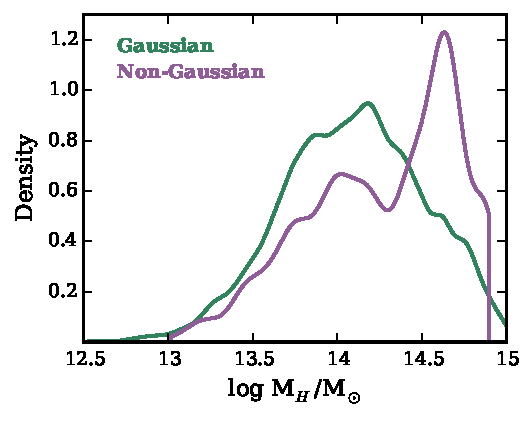
\includegraphics[width=\columnwidth]{mhdist_um.pdf}
  \caption{Smoothed host halo mass distributions for galaxies in the
    unmatched G and NG samples.}
  \label{fig:mhdist_um}
\end{figure}

To classify the dynamical state of the haloes in the data set we use a
combination of two statistical tests, the Anderson-Darling (AD)
normality test (\citealt{anderson1952}; see \citealt{hou2009, hou2013}
for an astronomical application) and the Dip test
(\citealt{hartigan1985}; see \citealt{ribeiro2013} for an astronomical
application).
\par
The AD test is a non-parametric test of normality based
upon the comparison between the cumulative distribution function (CDF) of a
measured data sample and the CDF of a gaussian distribution.  Under
the assumption that the data is in fact normally distributed, the AD
test determines the probability ($p$) that the difference between
the CDFs of the data and a normal distribution equals or exceeds the
observed difference.  We apply the AD test to the velocity
distributions of the member galaxies of each group in the data sample,
thereby broadly classifying the dynamical state of each halo.  All of
our groups have eight or more member galaxies, and 85 per cent of our
groups have five or more member galaxies within the virial radius.  Our
first criteria in classifying a group as Gaussian (G) is that the p-value given
by the AD test be greater than or equal to 0.05.
\par
Our second criteria required for a
group to be classified as G is that it be unimodal.  Ideally one would
hope that standard normality tests would detect all instances of
multimodality, however this is not always the case.  In particular,
multimodality in distributions with modes at small seperations
can be missed by standard statistical techniques \citep{ashman1994}. To
gauge the modality of the velocity distribution of a given group we
use the Dip test.  Like the AD test, the Dip test is also a
non-parametric CDF statistic.  Where they differ is that the Dip test
looks for a flattening of the CDF for the data which would correspond
to a `dip' in the distribution being tested.  The Dip test operates
under the null hypothesis that the data is unimodal, and we consider a
group velocity distribution unimodal if the Dip test p-value is
greater than or equal to 0.05.  Therefore our G data sample consists
of all those groups with $p_{\text{ad}} \ge 0.05$
\emph{and} $p_{\text{dip}} \ge 0.05$, whereas our non-Gaussian (NG) data
sample consists of all those groups with $p_{\text{ad}} < 0.05$
\emph{or} $p_{\text{dip}} < 0.05$.
\par
After applying the above criteria we find a G sample consisting of
$42\,655$ galaxies within $2\,447$ groups and a NG sample consisting of $5\,306$
galaxies within 215 groups.  We find that the AD test is the stronger discrimator
compared to the Dip test as out of all of the galaxies making up the
NG sample, 90 per cent failed the AD test but passed the Dip test, 8
per cent passed the AD test but failed the Dip test, and 2 per cent
failed both the AD test and the Dip test.  The authors note that it is
easier to statistically identify NG groups for groups with high
galaxy membership, this can lead to the NG sample being skewed toward
large halo masses (see Fig.~\ref{fig:mhdist_um}).  To address this we
match of G and NG samples by halo mass (as well as stellar mass and
redshift), as described in the following section.

\subsection{Matched data set}
\label{sec:match}

\begin{figure*}
  \centering
  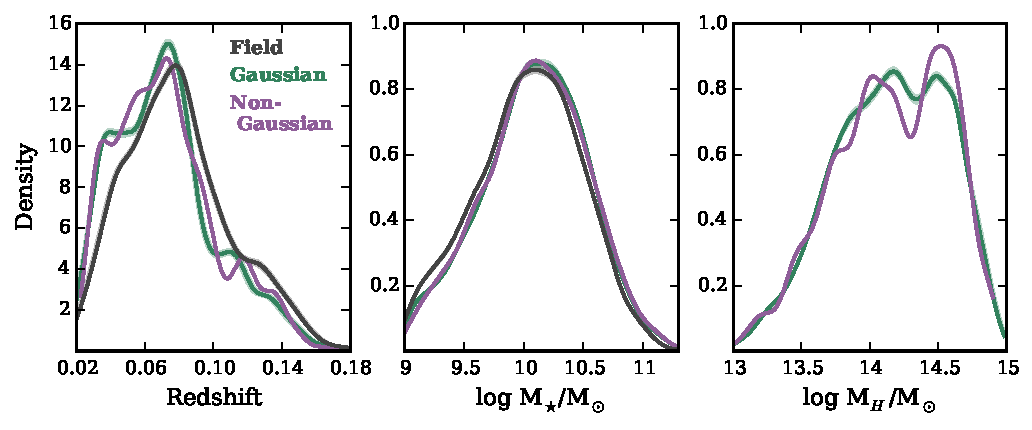
\includegraphics[width=\textwidth]{dist_m2_s.pdf}
  \caption{Smoothed distributions for stellar mass, redshift, and host
    halo mass for galaxies in the matched G, NG and field (where
    applicable) samples.  Shaded regions around the G and field lines
    are 90 per cent confidence intervals corresponding to the
    stochastic nature of our matching procedure.}
  \label{fig:dist_m2_s}
\end{figure*}

To ensure a fair comparison between galaxies in different environments
(ie.\ field galaxies, galaxies in G groups, and galaxies in NG groups)
we match our sample of G group galaxies and NG group galaxies by
stellar mass, redshift, and halo mass.  Additionally, we then match
our sample of field galaxies by stellar mass and redshift.  The
matching is particularly important when trying to elucidate
information on the effect of group dynamics on galaxy SF and
morphological properties for
two main reasons:
\par
First, stellar mass, redshift, and halo mass have
all been shown to influence galaxy SF and morphology
\citep[e.g.][]{brinchmann2004, feulner2005, zheng2007, cucciati2012,
  wetzel2012, lackner2013, tasca2014}; whereas
the impact of group dynamics is less clear \citep{hou2013,
  ribeiro2013} which is likely suggestive of a more modest role.
Therefore,
if one hopes to identify trends in galaxy SF and morphology with group
dynamics it is crucial to properly control for these other known correlations.
\par
Second, standard statistical normality tests, such as the AD test, are
biased towards identifying non-Gaussian distributions when
sample size is large.  This is a result of the statistical power of
the test increasing with sample size which subsequently allows the
detection of more and more subtle departures from normality
\citep{razali2011}.  While these subtle departures from normality will
perhaps be statistically significant, they may not be physically relevant (in
principle, no group is truly Gaussian) and what really matters is
whether galaxies in groups which show large departures from normality
have different properties than galaxies in groups which show smaller
departures from normality. Since group
richness generally scales with halo mass, in the absence of any matching
procedure, a sample of NG groups will be biased towards large halo
masses compared to a similar sample of G groups -- even though many
high halo mass NG groups may have been identified on the basis of very
small departures from normality.  Ensuring that our G and NG
samples have very similar halo mass distributions allows us to make a
fairer comparison between the two samples.
\par
Our algorithm for matching the G and NG samples is as follows:

\begin{enumerate}
  \item Our list of galaxies found in NG groups is iterated through,
    for each galaxy one `matching' galaxy from the G sample is
    found.  To be considered matching the two galaxies must have
    stellar masses within $0.1\,\mathrm{dex}$, redshifts within 0.01,
    and halo masses within $0.1\,\mathrm{dex}$.

  \item Step 1 is repeated until no more matches are
    found.  The end result is a list of galaxies from the NG
    sample each of which will have one or more matching galaxies from
    the G sample assigned to them
  
  \item The matched G sample is generated by including two galaxies
    from the G sample for every one matching galaxy from the NG
    sample.  By definition this excludes any galaxies in the NG
    sample which only have one identified match.  However, 85 per cent
    of galaxies
    in the NG sample have two or more matches so although we reduce
    the NG sample size by 15 per cent it allows us to increase the
    matched G sample size twofold.  It is worth noting that when we
    run our analysis keeping only one matched G galaxy instead of two,
    we find no changes in the trends observed.

  \item In the case where a given galaxy in the NG sample has more
    than two identified matches, the two matching galaxies from the G
    sample are
    chosen randomly.  This introduces a stochastic nature to our
    analysis as each generation of the matched G sample will not
    contain exactly the same galaxies.  To account for this, any
    quantities calculated using the matched G sample are done so in a
    Monte Carlo sense where the median of 1000 stochastic generations
    is quoted along with 90 per cent confidence intervals.
\end{enumerate}

\noindent
The field sample is subsequently matched to the NG sample following
the same procedure and the same method is used to account for the
stochastic nature of the matching procedure.  Fig.~\ref{fig:dist_m2_s}
shows smoothed density
distributions of stellar mass, redshift, and halo mass for the matched
G, NG, and field samples.  For the remainder of the
paper all analysis is done using the matched samples, therefore from
this point forward any reference to the G, NG, or field samples refers
to the matched samples.

%%%%%%%%%%%%%%%%%%%%%%%%%%%%%%%%%%%%%%%%%%%%

\section{Identifying infalling and virialized galaxies}
\label{sec:rad_div}

\begin{figure}
  \centering
  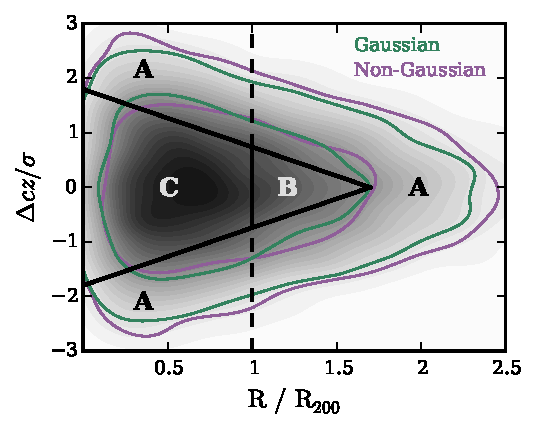
\includegraphics[width=\columnwidth]{vnorm_r_con.pdf}
  \caption{Projected radial phase space
    for galaxies within the group sample.  Grey shading shows the phase
    space density distribution for all group galaxies, green and
    purple contours correspond to the 68 and 95 per cent density
    regions for G and NG galaxies respectively. Virialized (C),
    backsplash (B), and infalling (A) regions using the cuts defined in
    \citet{mahajan2011} are shown.}
  \label{fig:vnorm_r}
\end{figure}

Galaxies within group haloes can be broadly classified into three main
subclasses: galaxies infalling to the group at large radii, galaxies
virialized within the inner regions of the halo, and galaxies
backsplashing beyond the virial radius after making a passage through
the group centre.  In order to understand the radial dependence of
galaxy properties within groups it is crucial to be able to
identify these different galaxy populations
\citep{gill2005, mahajan2011, pimbblet2011, haines2015, noble2016}.
\par
One method used to distinguish between infalling, virialized, and
backsplash populations is to look for distinct populations in radial
phase space.  In particular \citet{mahajan2011} follow
\citet{sanchis2004} and identify galaxies within one virial radius as
virialized and use the cut

\begin{equation} \label{eq:cut}
  \frac{v_r}{V_\mathrm{v}} = -1.8 + 1.06
  \left(\frac{r}{R_\mathrm{v}}\right)
\end{equation}

\noindent
to distinguish between infalling and backsplash galaxies.  Where $v_r$
is the radial velocity of the galaxy, $V_\mathrm{v}$ is the velocity
dispersion of the group, $r$ is the group-centric radius, and
$R_\mathrm{v}$ is the virial radius of the group.
\par
The cuts described above were determined using full 6-d phase space
information in simulations, however observationally we are limited to
line-of-sight
velocities and projected radii.  Although working in projection
removes much of the distinct phase space structure \citep{oman2013, haines2015},
density contours for the virialized, backsplash, and infalling
populations still occupy similar regions in projected phase space
with the contamination between different populations being more substantial
\citep{mahajan2011}.  While the divisions between populations is
certainly less clear in projection, equation~\ref{eq:cut} can still be
used to obtain an approximate division between infalling, virialized,
and backsplash galaxies -- this approximation is preferred over
the incorrect assumption that all galaxies beyond the virial radius
are infalling for the first time.  In particular, at intermediate
radii, $1 < R < 1.5\,\mathrm{R_{200}}$, as much as 60 per cent of the
galaxy population could be backsplashing \citep{mahajan2011, hou2014}.
\par
To make the transformation to observational quantities we replace
$v_r/V_\mathrm{v}$ with $\Delta cz/\sigma$ and $r/R_\mathrm{v}$ with
$R/R_{200}$ in equation~\ref{eq:cut}.  We also symmetrize the phase
space cuts to account for projection by using the mirror of
equation~\ref{eq:cut}.  After implementing these observational
adjustments, and utilizing the best-fitting scheme from
\citet{mahajan2011}, we show the phase space distribution of the total
group sample, as well as galaxies in G and NG groups, in
Fig.~\ref{fig:vnorm_r}.  In addition, we divide the phase space into
the infalling (Regions A), backsplash (Region B), and 
virialized (Region C) populations. 

%%%%%%%%%%%%%%%%%%%%%%%%%%%%%%%%%%%%%%%%%%%%

\begin{figure*}
  \centering
  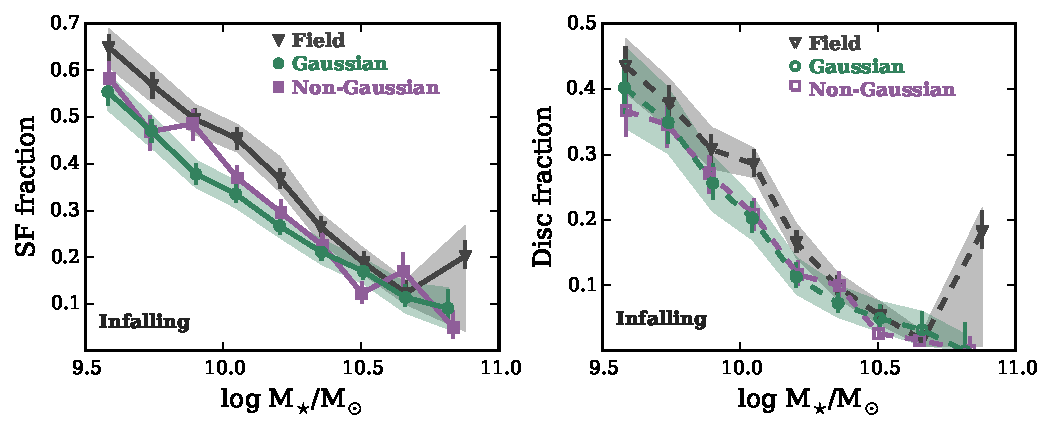
\includegraphics[width=\textwidth]{disk_sfFrac95_w2_if.pdf}
  \caption{Star forming (left) and disc (right) fraction versus stellar mass for
    field galaxies as well as infalling galaxies in the G and NG
    samples.  Error bars correspond to $1 \sigma$ binomial confidence
    intervals as given in \citet{cameron2011}, shaded regions are 90
    per cent Monte Carlo confidence intervals derived from the
    stochastic nature of the matching procedure for the G and field samples.}
  \label{fig:disk_sfFrac_if}
\end{figure*}

\section{Galaxy properties in the infall region}
\label{sec:infall}

We first consider the star-forming and morphological properties of
galaxies infalling (Regions A in Fig.~\ref{fig:vnorm_r}) onto both G
and NG groups, as well as galaxies within the field sample.  We apply
a lower stellar mass cut at $10^{9.5}\Msun$ in order to avoid
including galaxies with large $1/V_\mathrm{max}$ weights.  In
Fig.~\ref{fig:disk_sfFrac_if} we plot star-forming and disc fraction
of infalling galaxies
versus stellar mass for the three different galaxy samples.  We define
star-forming galaxies to be all galaxies with $\log SSFR \ge -11$,
\citet{wetzel2012} show that in the local Universe the division
between the red sequence and the blue cloud is consistently found at
$\log SSFR \simeq -11$ across a wide range of halo masses.  Likewise
we define disc galaxies to be all galaxies having a global S\'{e}rsic
index of $n \le 1.5$.  While the distribution of S\'{e}rsic index is
not as clearly bimodal as the SSFR distribution, we find that our
observed trends are insensitive to our exact choice of dividing S\'{e}rsic
index.
\par
Inspection of Fig.~\ref{fig:disk_sfFrac_if} reveals certain
interesting features.  First, there is no significant difference
between the star-forming or disc fractions for galaxies infalling onto
G groups compared to galaxies infalling onto NG
groups.  This suggests that any influence that the dynamical state
of the group
has on star forming or morphological properties is not in place during
a galaxies first infall toward the virialized region of the halo.
Additionally very similar trends are observed for both star-forming and
disc fractions.
\par
We also see only a small excess of star-forming galaxies in the field
compared to galaxies falling into haloes.  When looking at disc fraction, this
``field excess'' is very marginal.
Previous studies \citep{lewis2002, gray2004, rines2005, verdugo2008}
have found that star formation of galaxies within infall regions
remains suppressed compared to the field out to radii on the order of
$2-3\,R_{200}$.  This suppression is often attributed to
backsplash galaxies which have already made a passage through the halo
centre, the pre-processing of galaxies in small groups prior to
infall, or some combination of the two.  Using the cuts described in
Section~\ref{sec:infall} we have attempted to ``clean'' our infall sample
of backsplashing galaxies, although there is still some level of
contamination due to the lack of full phase space information.
\par
It is expected that pre-processing
should play a more important role in large clusters compared to smaller
groups, as a larger fraction of galaxies infalling onto clusters will
have been a part of a group prior to infall.  This is
simply a result of the hierarchical build-up of structure and the
fact that regions of space around large clusters are not average but
are preferentially populated with other dense structures such as group
haloes \citep[e.g.][]{mo1996, wang2008}.

\begin{figure}
  \centering
  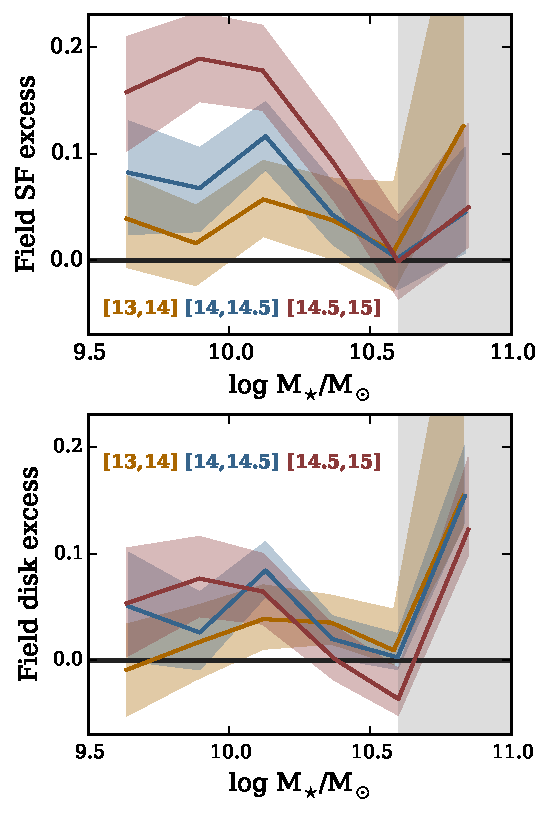
\includegraphics[width=\columnwidth]{mh_excess95.pdf}
  \caption{The excess in star-forming (top) and disc (bottom) fraction
  for galaxies in the field versus galaxies in the infall region of
  groups.  We show field excess versus stellar mass for three
  different halo mass ranges: $10^{13} < M_H \le 10^{14}\Msun$ (goldenrod),
  $10^{14} < M_H \le 10^{14.5}\Msun$ (blue), and $10^{14.5} < M_H \le
  10^{15}\Msun$ (red).  Shaded bands indicate $1\sigma$ statistical
  errors \citep{cameron2011}, the region at high stellar mass shaded
  in gray indicates where Monte Carlo errors from our matching
  procedure become large compared to the statistical uncertainties.}
  \label{fig:mh_excess}
\end{figure}

We look for evidence of pre-processing by examining the ``field
excess'', which we define as the difference in star forming or disc
fraction between field galaxies and galaxies infalling into haloes,
for different halo mass ranges.  Specifically, we split our group
sample into three halo mass bins: $10^{13} < M_H \le 10^{14}\Msun$,
  $10^{14} < M_H \le 10^{14.5}\Msun$, and $10^{14.5} < M_H \le
  10^{15}\Msun$.  Since we see no strong
differences between infalling galaxies for G and NG groups in any of
our halo mass bins, we measure field excess with
respect to the star-forming and
disc fractions of all infalling galaxies regardless of whether they
are infalling onto a G or NG group.  In Fig.~\ref{fig:mh_excess}  we show
the field excess, in star-forming fraction and disc
fraction, and its dependence on halo mass.  We see that field excess
tends to increase with halo mass, with a star-forming field excess of
up to $\sim\!15$ per cent in rich clusters.  This trend is clearest when
considering star-forming fraction and it is less obvious when
considering disc fraction -- though we do still 
see an excess of disc galaxies compared to the field for the higher
halo masses.  The observed field excess is consistent with pre-processing, as
the expected relatively high degree of pre-processing of galaxies falling into
clusters would drive a larger deviation from the field population, and
similarly the lower expected levels of pre-processing for smaller
groups would lead to a smaller difference between galaxies infalling into
these groups and galaxies in the field.  In Fig.~\ref{fig:mh_excess}
we shade in gray a region at high stellar mass where a sharp upturn is
observed, we do this to highlight that at these masses the Monte Carlo
uncertainty due to the stochastic nature of our matching procedure is
large compared to the statistical errors (see
Fig.~\ref{fig:disk_sfFrac_if}) and therefore this upturn could simply
be a result of random fluctuations.

%%%%%%%%%%%%%%%%%%%%%%%%%%%%%%%%%%%%%%%%%%%%%%

\section{Galaxy properties in the virialized region}
\label{sec:virial}

\begin{figure*}
  \centering
  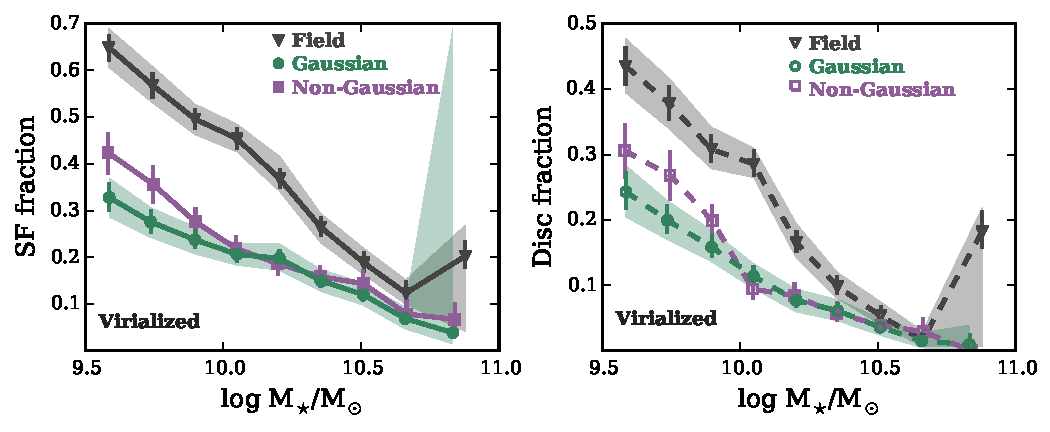
\includegraphics[width=\textwidth]{disk_sfFrac95_w2_v.pdf}
  \caption{Star-forming (left) and disc (right) fraction versus stellar mass for
    field galaxies as well as virialized galaxies in the G and NG
    samples.  Error bars correspond to $1 \sigma$ binomial confidence
    intervals as given in \citet{cameron2011}, shaded regions are 90
    per cent Monte Carlo confidence intervals derived from the
    stochastic nature of the matching procedure.}
  \label{fig:disk_sfFrac_v}
\end{figure*}

We now consider star-forming and disc fractions for galaxies within
the virialized region of the halo (Region C in
Fig.~\ref{fig:vnorm_r}), and again consider the differences between
the G, NG, and field samples.  Fig.~\ref{fig:disk_sfFrac_v} shows
star-forming and disc fractions versus stellar mass for the three
galaxy samples.  In contrast to the infalling region, when
considering star-forming and
disc fractions for galaxies within the virialized region of the halo a
subtle dependence 
on group dynamics emerges.  In particular, galaxies in G groups have
the lowest star-forming and 
disc fractions, and galaxies in NG groups have intermediate
values -- larger star forming and disc fractions than galaxies in G
groups but significantly smaller than galaxies in the field.
Moreover, we only observe this difference between the G and NG samples
for galaxies $\la 10^{10}\Msun$, for stellar masses higher than this
threshold no dependence on group dynamics is observed.  As with the
infalling region (Fig.~\ref{fig:disk_sfFrac_if}), we see qualitatively
similar trends in both star forming and disc fractions.

%%%%%%%%%%%%%%%%%%%%%%%%%%%%%%%%%%%%%%%%%%%

\section{Discussion}
\label{sec:discussion}

\subsection{The impact of group dynamical state}

The question of to what degree group dynamical state influences galaxy
properties is one which has not yet been conclusively answered.  In
this study we find that properties of low-mass galaxies within the inner
regions of haloes show a dependence on group dynamics.  In
particular, we find that galaxies in the virialized region of NG
groups show an increase in both star-forming and disc fractions
when compared to galaxies in the same region of G groups.
\par
\citet{carollo2013} study the differences between galaxies in
`relaxed' and `unrelaxed' groups (defined based upon the presence, or
lack thereof, of a well defined central group galaxy) in the Zurich
Environmental Study.  \citet{carollo2013} find that $<10^{10}\Msun$
satellites show slightly redder colours in relaxed groups compared to
unrelaxed groups.  Given the general correlations between galaxy colour, star
formation, and morphology, this agrees well with the findings of this
work. \citet{ribeiro2013} use a statistical metric designed to quantify the
distance between probability density functions, known as the Hellinger
distance, to discriminate between G and NG groups using a
FOF catalogue of SDSS group galaxies
\citep{berlind2006}.  They find no dependence on group dynamics for
bright galaxies ($\mathrm{M_r} \le -20.7$), however find that
properties of faint galaxies ($-20.7 < \mathrm{M_r} \le -17.9$) do
depend on whether they live in a G or NG group.  Relevant to this
work, \citet{ribeiro2013} show that faint galaxies in G groups are
redder than their NG counterparts. As well Ribeiro et al. calculate
mean colours for galaxies in the inner and outer region of the halo
(dividing the inner and outer halo at the median radius) for G and NG
groups.  They find that the colours of galaxies in NG groups do not
change radially, but galaxies in the inner region of G groups are
redder than those in the outer region.
\par
The results of this paper can be used to further constrain the
connection between group dynamics and the quenching of star formation as well
as morphological transformations.  The main result that we observe a
dependence on dynamics in the virialized region of the halo but not
for galaxies infalling for the first time seems to suggest quenching and
morphological transformations primarly take
place within the virial radius, and are more efficient in G
groups than NG groups.  Alternatively, the observed excess of
star-forming, disc galaxies in NG groups could be due to the more
dynamically complex NG groups having assembled more recently,
therefore galaxies in G groups will have been exposed to quenching
mechanisms within the group environment for longer.  Examination of
Fig.~\ref{fig:disk_sfFrac_v} shows that very similar trends are observed
between the virialized G and NG populations when considering either
star formation or morphology.

\subsection{Pre-processing of infalling galaxies}

\begin{figure}
  \centering
  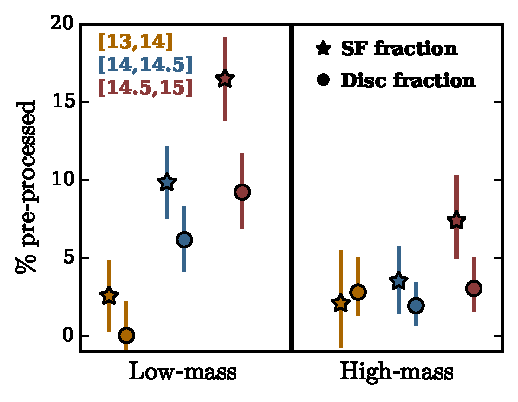
\includegraphics[width=\columnwidth]{pp_mh.pdf}
  \caption{Pecentage of infalling galaxies which have had
    star-formation (stars) or morphology (circles) pre-processed for
    both low-mass ($M_\star \la 10^{10.3}\Msun$, filled markers) and 
  high-mass ($M_\star \ga 10^{10.3}\Msun$, open markers) galaxies, as
  a function of halo mass.  Error bars correspond to $1\sigma$
  binomial confidence intervals \citep{cameron2011}.}
  \label{fig:pp_mh}
\end{figure}

In addition to star formation quenching and morphological
transformations within the current host halo, we also find evidence
for pre-processing in both star formation and morphology.  To probe
pre-processing we measure the ``field excess'' (ie.\ the degree to
which star-forming and disc fractions are enhanced in the field
relative to the infalling region of groups).  Assuming that any
environmentally driven quenching or morphological transformations occur within the virialized region of a halo,
then the field excess will just correspond to the fraction of
infalling galaxies which have been pre-processed.  Using this we
quantitatively determine the level of pre-processing by computing the
field excess for low-mass ($M_\star \la
10^{10.3}\Msun$) and high-mass  ($M_\star \ga 10^{10.3}\Msun$)
galaxies in our three halo mass bins.  In Fig.~\ref{fig:pp_mh} we plot
the fraction of low-mass and high-mass infalling galaxies which have
had star formation or morphology pre-processed.  We further divide into
bins of halo mass to display the halo mass dependence of
pre-processing.  Both star formation and morphology are pre-processed,
with the fraction of pre-processed galaxies ranging between $\sim\!0$
and $\sim\!15$ per cent when considering star-forming fraction and
$\sim\!0$ and $\sim\!10$ per cent when considering disc fraction,
depending on stellar and halo mass.  Low-mass
galaxies show stronger pre-processing than their high-mass
counterparts and the
strength of pre-processing increases with halo mass. 
\par
Prior studies have aimed to constrain the
fraction of pre-processed galaxies both observationally and using
simulations.  One common approach is to measure the fraction of
galaxies which fall onto a cluster as a member of a smaller group,
either directly using simulations or by measuring substructure or
clustering observationally.  For clusters with mass $\sim
\!10^{14}\Msun$ \citet{delucia2012} use semi-analytic models (SAMs) and find
that the fraction of satellite galaxies which are accreted in groups
with $M_H \ga 10^{13}\Msun$ is highest for low-mass galaxies,
corresponding to $\sim\!28$ per cent.  Also using SAMs,
\citet{mcgee2009} find that the fraction of galaxies accreted onto the
ultimate cluster as members of $\ga 10^{13}\,h^{-1}\Msun$ groups depends
strongly on the cluster halo mass, ranging from $\sim\!0.1$ for
$10^{13.5}\,h^{-1}\Msun$ haloes to $\sim\!0.45$ for haloes with masses
of $10^{15}\,h^{-1}\Msun$.  \citet{bahe2013} use the \textsc{gimic}
suite of zoom in simulations and find that the fraction of galaxies
which have been satellites of a $>\!10^{13}\Msun$ halo prior to accretion
onto the ultimate host ranges from $<10$ per cent for a host with halo
mass $<\!10^{13.5}\Msun$, up to as high as $\sim\!60$ per cent for a
host halo mass of $10^{15.2}\Msun$.
Observationally, \citet{hou2014} use the
Dressler-Schectman test \citep{dressler1988} to identify infalling
subhaloes and find for $<\!10^{14}\Msun$ groups that less than 5 per
cent of infalling galaxies are part of a subhalo, whereas for haloes
with masses $10^{14} < M_H < 10^{14.5}\Msun$ and $M_H >
10^{14.5}\Msun$ the fraction of galaxies infalling in subhaloes is
$\sim 10$ per cent and $\sim 25$ per cent, respectively.
Qualitatively the pre-processing trends observed in this work are
consistent with these previous studies, namely the fraction of
pre-processed galaxies tends to decrease with increasing galaxy stellar mass and
increase with the halo mass of the host which the galaxies are
infalling onto.  The subhalo fraction found in these works is
essentially an upper limit on the field excess quantity which we
quote.  This is because only some fraction of galaxies within subhaloes
during infall will actually have been pre-processed, whereas the
field excess more closely measures the fraction of galaxies
which have actually been pre-processed.  Therefore the fact that our
values for the fraction of pre-processed galaxies are consistently
smaller than the quoted subhalo fractions is entirely consistent.
\par
Studying the star-forming fractions of cluster galaxies,
\citet{haines2015} use a simple toy model in an attempt to reproduce the
trend between cluster-centric radius and star-forming fraction.  They
find that in order to reproduce the observational trend, a $19$ per
cent decrease in the star-forming fraction of cluster galaxies relative to
the field is required on top of star
formation quenching occuring within the virial radius.  Haines et
al. suggest that pre-processing is a possible mechanism to generate
this $19$ per cent decrease.  In this work we find that the fraction of
high-mass (the Haines et al. sample consists of galaxy stellar masses
$>\!2 \times 10^{10.2}\Msun$) pre-processed galaxies for high-mass
clusters is $8 \pm 3$ per cent.  Therefore, this work is not able to
account for the amount of pre-processing required by the
\citet{haines2015} model.
\par
At $\sim\!z=0.2$, \citet{lu2012} find that blue fractions of low and
intermediate-mass cluster galaxies are lower than the field values
(for the appropriate stellar mass) out to radii of $7\,\mathrm{Mpc}$, however
the most massive galaxies
show no difference from the field.  This is similar to the stellar
mass trends observed in this work where we only see strong
pre-processing for low-mass galaxies.
\par
Evidence for the pre-processing of both star formation and/or morphology is
something that has been seen in recent literature, and seeing as we detect the
pre-processing of
both star formation and morphology in this work it is interesting to
compare the level of pre-processing between the two.  In
general we find that the fraction of low-mass galaxies which have been
morphologically pre-processed is slightly smaller than the fraction of
low-mass galaxies which have had their star formation pre-processed,
this is consisent across our different halo mass bins.

%%%%%%%%%%%%%%%%%%%%%%%%%%%%%%%%%%%%%%%%%%%

\section{Summary \& conclusions}
\label{sec:summary}

In this paper we investigate the dependence of galaxy properties
(namely, star-forming and disc fractions) on host group dynamics.  To
do so we construct a carefully matched sample of galaxies housed in
Gaussian groups, galaxies housed in non-Gaussian groups, as well as
field galaxies; all with similar distributions in stellar mass,
redshift, and (field galaxies excluded) halo mass.  We then compare
the properties of these different samples for two different regions
within the halo: the infalling region, and the virialized region.  The
main findings of this work are as follows:

\begin{enumerate}
  \item Star-forming and disc fractions of infalling galaxies do not
    depend on the dynamics of the group that they are falling onto.

  \item We detect pre-processing by measuring the difference between
    the star-forming and disc fractions for field galaxies compared to
    infalling galaxies.  Infalling galaxies have had both star
    formation and morphology pre-processed, with low-mass galaxies
    infalling onto high-mass haloes showing the largest degree of
    pre-processing.

  \item Galaxies in the virialized region of the halo show a clear
    dependence on group dynamical state.  Low-mass galaxies in
    non-Gaussian groups show enhanced star-forming and disc fractions
    compared to galaxies in Gaussian groups at the same stellar mass. 
\end{enumerate}

%%%%%%%%%%%%%%%%%%%%%%%%%%%%%%%%%%%%%%%%%%

\section*{Acknowledgments}
\label{sec:acknowledgments}

IDR thanks the Ontario Graduate Scholarship program for funding.  LCP
thanks the National Science and Engineering Research
Council of Canada for funding.  The authors thank
F. Evans for matching together the various SDSS catalogues used in
this research.  We thank X. Yang et al. for
making their
SDSS DR7 group catalogue publicly available, L. Simard et al. for the
publication of their SDSS DR7 morphology catalogue, J. Brinchmann et al. for
publication of their SDSS SFRs, and the NYU-VAGC
team for the 
publication of their SDSS DR7 catalogue.  This research would not have
been possible without access to these public catalogues.
\par
Funding for the SDSS has been provided by the Alfred P. Sloan
Foundation, the Participating Institutions, the National Science
Foundation, the U.S. Department of Energy, the National Aeronautics
and Space Administration, the Japanese Monbukagakusho, the Max Planck
Society, and the Higher Education Funding Council for England. The
SDSS Web Site is http://www.sdss.org/.
\par
The SDSS is managed by the Astrophysical Research Consortium for the
Participating Institutions. The Participating Institutions are the
American Museum of Natural History, Astrophysical Institute Potsdam,
University of Basel, University of Cambridge, Case Western Reserve
University, University of Chicago, Drexel University, Fermilab, the
Institute for Advanced Study, the Japan Participation Group, Johns
Hopkins University, the Joint Institute for Nuclear Astrophysics, the
Kavli Institute for Particle Astrophysics and Cosmology, the Korean
Scientist Group, the Chinese Academy of Sciences (LAMOST), Los Alamos
National Laboratory, the Max-Planck-Institute for Astronomy (MPIA),
the Max-Planck-Institute for Astrophysics (MPA), New Mexico State
University, Ohio State University, University of Pittsburgh,
University of Portsmouth, Princeton University, the United States
Naval Observatory, and the University of Washington.

%%%%%%%%%%%%%%%%%%%%%%%%%%%%%%%%%%%%%%%%%%%%%%%%%%

%%%%%%%%%%%%%%%%%%%% REFERENCES %%%%%%%%%%%%%%%%%%

% The best way to enter references is to use BibTeX:

\bibliographystyle{mnras}
\bibliography{RobertsParker2016} % if your bibtex file is called example.bib


% Alternatively you could enter them by hand, like this:
% This method is tedious and prone to error if you have lots of references
%\begin{thebibliography}{99}
%\bibitem[\protect\citeauthoryear{Author}{2012}]{Author2012}
%Author A.~N., 2013, Journal of Improbable Astronomy, 1, 1
%\bibitem[\protect\citeauthoryear{Others}{2013}]{Others2013}
%Others S., 2012, Journal of Interesting Stuff, 17, 198
%\end{thebibliography}


% Don't change these lines
\bsp	% typesetting comment
\label{lastpage}
\end{document}

% End of mnras_template.tex
